\section{Class Inheritance and Dependencies}
As described in the previous section, classes are organised into packages. The design of the packages group together classes of certain types. Classes in a package are expected to depend on and interact with classes in the same package and with classes in other packages.\\
It is virtually impossible to produce and include a UML class diagram of this application and have it fit on a piece of portrait A4. So the following UML diagram shows all of the classes and their packages, albeit without methods and attributes (Significant class methods are listed in Section 3), and shows the dependencies between facades and entities, and the dependencies of the FriendsServlet for example.

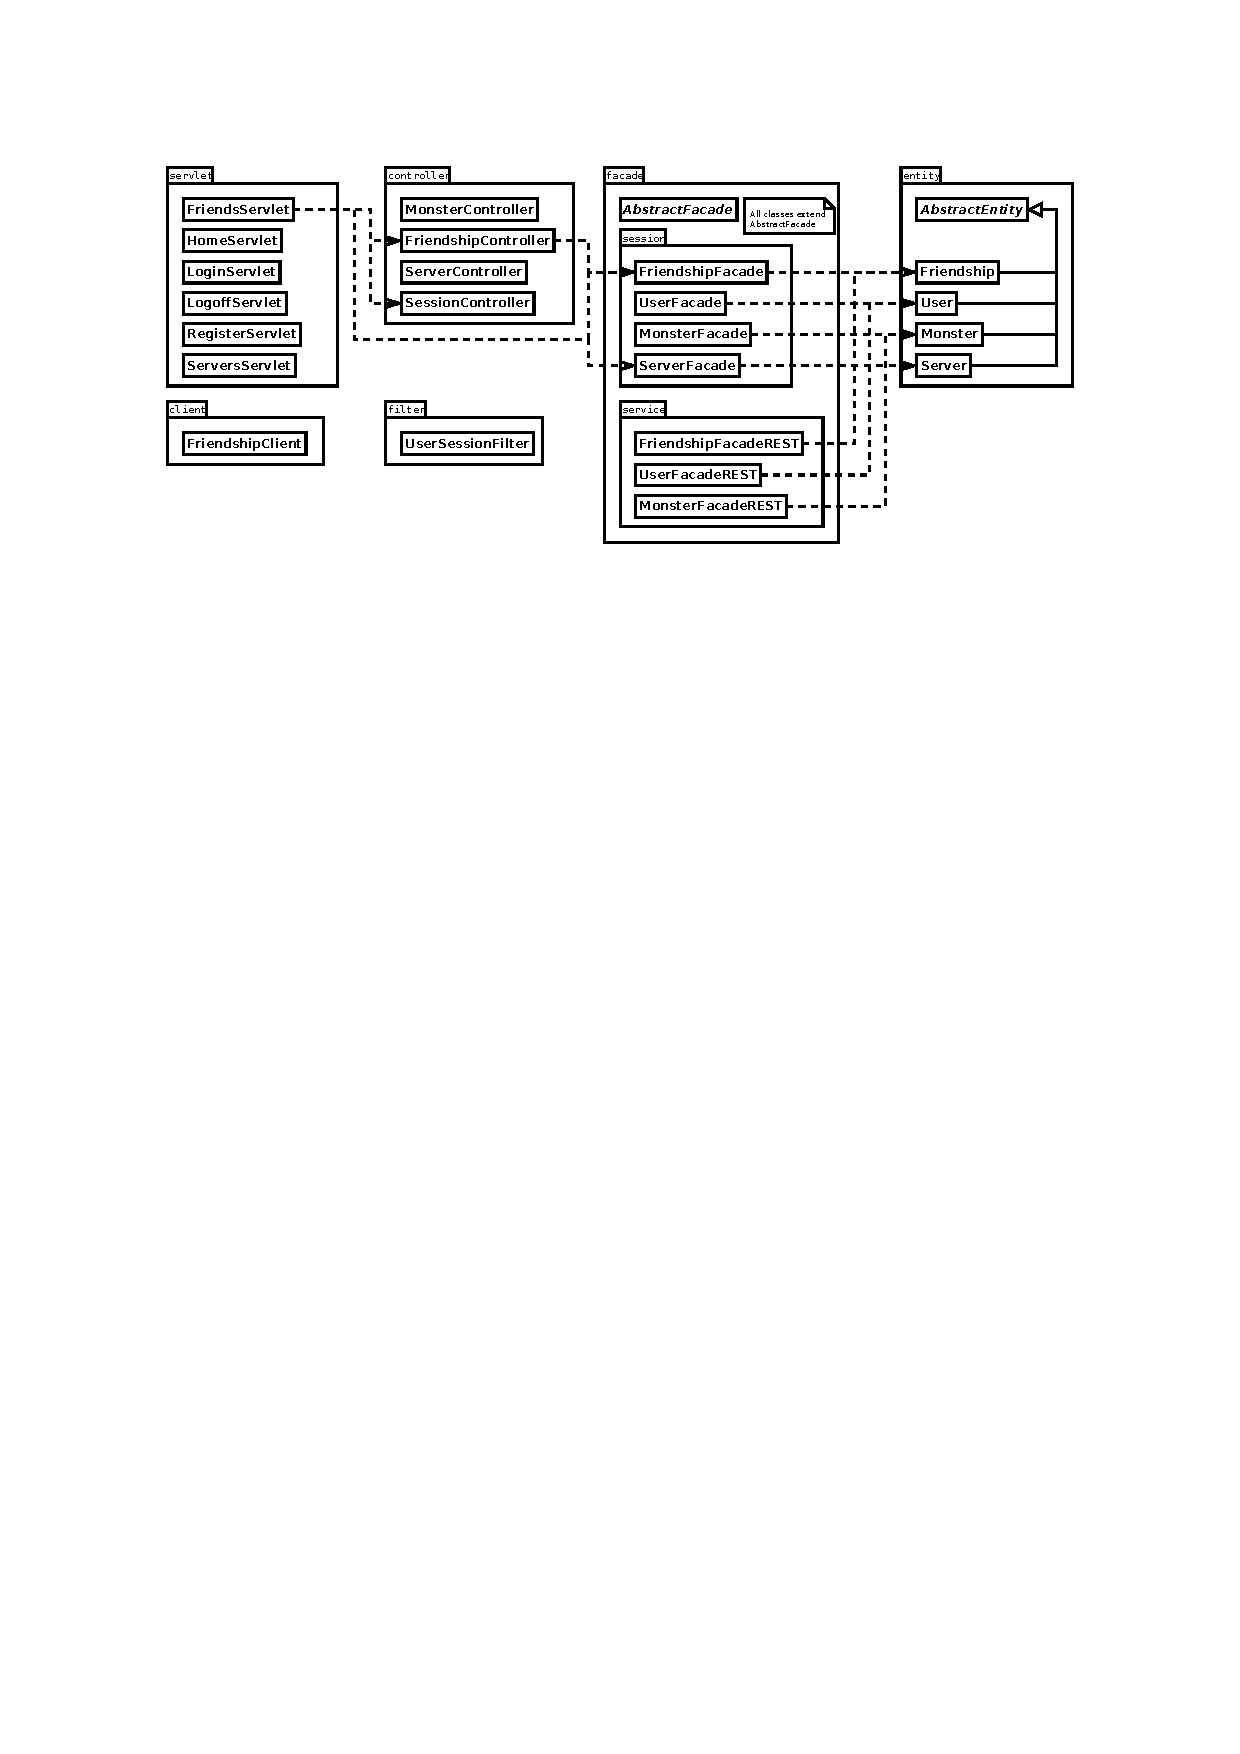
\includegraphics[scale=1.0]{img/dependencydiagram.pdf}

While we cannot deliver a complete UML diagram, we can describe a few design facts:
\\
\begin{itemize}
\item All entity classes have a corresponding session Facade class, so User will have UserFacade
\item The retrieval and persistence of Entity objects will be done via the Entity class' corresponding Facade class.
\item An Entity object, once it has been created, or obtained from a Facade, can be directly manipulated using it's accessors. The changes to that Entity object can then be persisted back to the database by passing it to the appropriate methods in the Entity's corresponding Facade.
\item There does not have to be a 'service' facade for each entity, only if the entities will be accessed via the ReST protocol
\item Controllers are stand-alone objects, in that they do not inherit from any other class
\item There will be a separate controller class for each entity, should one be required
\item Controller and Facade classes can depend on and interact with other controllers and facades, so that multiple types of entities can be used in the same place
\item Servlets can access and manipulate entity objects via corresponding controllers, facades, or a mixture of both
\item All Servlets extend the Java EE abstract class \textit{HttpServlet} and should override \textit{doGet} and if appropriate \textit{doPost}
\item Servlets should not depend on or interact with other servlet classes
\item Instances of Controller and Facade classes should be 'injected' into a depending class via EJB. In other words, a controller or a facade should not be instantiated when it is required by say a servlet for example. A single shared session instance of the classes should be obtained by using the \textbf{@EJB} annotation.
\end{itemize}

\clearpage
%\subsection{Servlet mapping and dependencies}
%This subsection lists every browsable page in the application, it's corresponding servlet, and which classes each servlet depends on.\\
%\begin{tabular}{|p{3cm}|p{3cm}|p{10cm}|}
%\hline
%\textbf{Web page}			& \textbf{Servlet}		& \textbf{Dependencies} \\
%\hline
%User's friends				& FriendsServlet		& FriendshipController, FriendshipFacade, ServerFacade \\
%\hline
%\end{tabular}

